\documentclass{article}

% Device-track application (CoRL 2026 workshop "The UMI Arena", Track 2):
% 2-4 pages + a 1-3 min video. Not double-blind: the device is brought in
% person. 'preprint' shows authors and drops the CoRL footnote.
\usepackage[preprint]{corl_2026}
\usepackage{graphicx}
\usepackage{booktabs}
\usepackage{xcolor}
\usepackage{siunitx}
\newcommand{\todo}[1]{\textcolor{red}{[#1]}}

\title{YAM-UMI: A Fiducial-Tracked Glove that Collects\\Metrically Labelled Demonstrations for the YAM}

\author{
  Yosub Shin \\
  University of Hawaii at Manoa \\
  \texttt{yosubs@hawaii.edu} \\
  \And
  Yuan Liu \\
  Independent \\
  \texttt{hiveyuan@gmail.com} \\
  \And
  Igor Molybog \\
  University of Hawaii at Manoa \\
  \texttt{molybog@hawaii.edu} \\
}

\begin{document}
\maketitle

%===============================================================================
\begin{abstract}
YAM-UMI is a glove-style UMI gripper that replicates the I2RT YAM linear gripper and is tracked by printed fiducials rather than an inertial camera: an 11-face ball on the back of the hand, seen by one fixed 4K camera over the workspace, gives the pose, and two tags in the jaws, seen by the glove's wrist fisheye, give the width. No IMU and no SLAM, so no drift: every label is an absolute per-frame measurement with a known error: the same stack mounted on the robot disagrees with the robot's kinematics by \SI{7.7}{mm} / \SI{1.7}{\degree} median, and policies trained on its labels instead of robot ground truth pay a constant \SI{14}{\percent} in validation loss. One person records 2.6--2.9 demonstrations per minute with the glove against 0.9--1.1 by teleoperation. Adding 165 glove episodes to 185 teleoperated ones lowers ACT's validation loss on the robot's held-out episodes (0.260 vs 0.295 forward camera, 0.236 vs 0.247 wrist) and in 30 paired rollouts per policy the co-trained wrist policy grasps the block as often as the teleop-only one (28/30 against 26/30), but neither co-trained policy measurably changes success (14/30 and 12/30 against 16/30, n.s.); replacing half or three quarters of the teleoperated episodes with glove episodes at the same budget costs 33--37 points ($p<0.01$). Hardware and software are open; three units have been built from the files, one independently by a third party.
\end{abstract}
\begin{figure}[t]
  \centering
  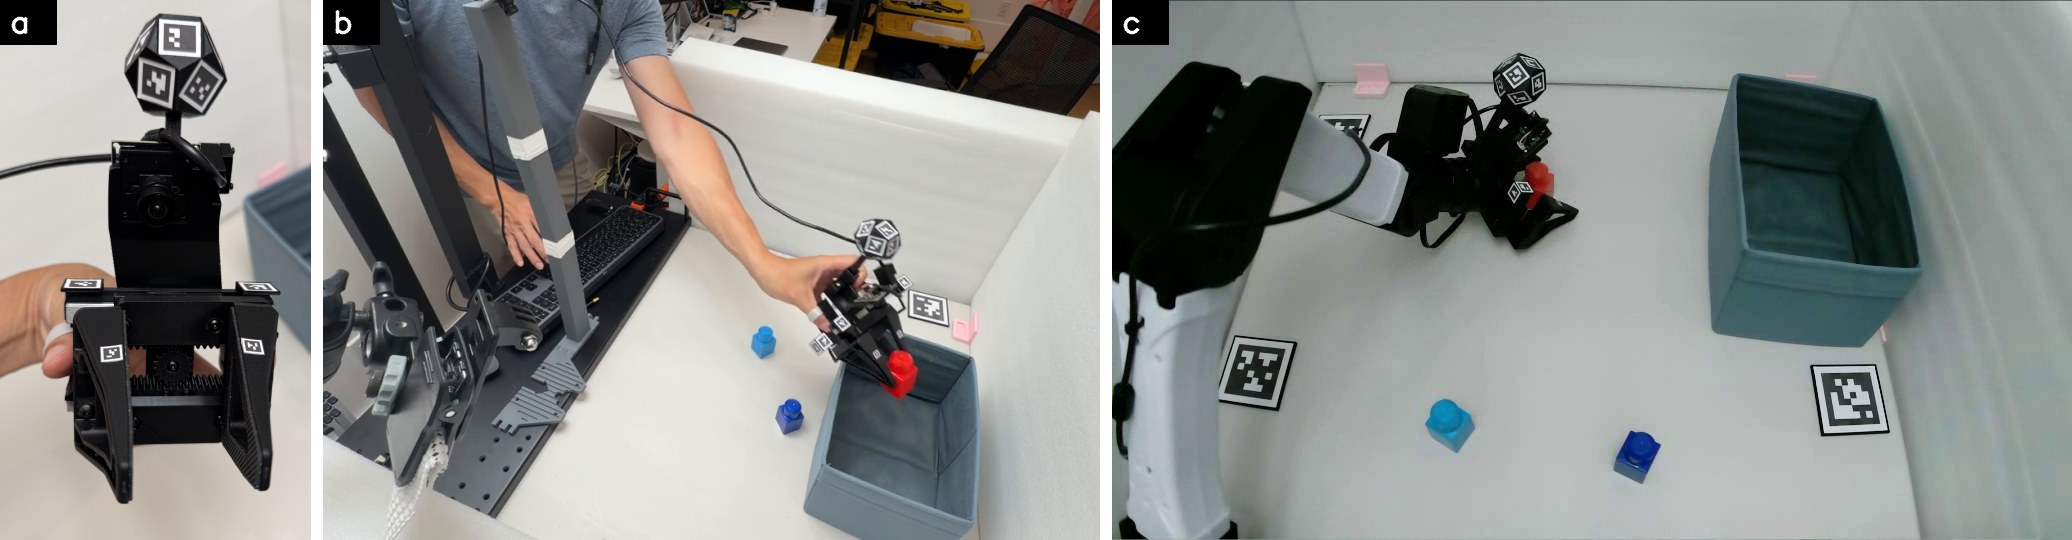
\includegraphics[width=0.92\linewidth]{fig/teaser.jpg}
  \vspace{1pt}
  {\footnotesize
  \begin{tabular}{@{}p{1.85cm}p{12.4cm}@{}}
    \toprule
    \textbf{Ergonomics} & \SI{355}{g} on the hand with cable (\SI{318}{g} without), under half of UMI's \SI{780}{g}; nothing to initialise. \\
    \textbf{Dexterity} & the YAM gripper's tasks (parallel-jaw pick, place, insert); \SI{0}{}--\SI{75}{mm} opening, robot's own fingers. \\
    \textbf{Strength} & \SI{1}{kg} by a jug handle, \SI{1.5}{kg} slips, \SI{2}{kg} no (robot: \SI{1.5}{kg}/\SI{2}{kg}); MGN9 rails, no wear in a month. \\
    \textbf{Reproducibility} & hardware and software open; one two-plate print, 7 purchased parts; three units built, one by others. \\
    \textbf{Cost} & \$79 per glove (\$22 without wrist camera); \$122 of shared rig; $\sim$\$200 per system vs UMI's \$371. \\
    \bottomrule
  \end{tabular}}
  \caption{(a) The glove: the robot's gripper fingers on a printed body, fiducial ball, marker cubes, wrist fisheye. (b) Collecting under the fixed 4K camera that labels the pose every frame. (c) A co-trained policy on the YAM, carrying the same ball that validated the labels. Below: the device against the workshop track's criteria.}
  \label{fig:teaser}
\end{figure}

%===============================================================================
\section{The device}
\label{sec:device}

\paragraph{Principle.}
The glove reproduces the robot's own parallel-jaw gripper \citep{i2rtyam}: the same \SI{95}{mm}-throw linear mechanism on two MGN9 rails, driven by a rack and pinion from a handle the operator squeezes, with the robot's own gripper fingers. All sensing is printed paper. A dodecahedral ball with eleven \SI{15}{mm} ArUco faces on the back of the hand gives the pose; two \SI{6}{mm} AprilTags in the jaws give the width to a wrist-mounted \SI{160}{\degree} fisheye; marker cubes on the jaws and four back markers keep the fixed camera tracking when the hand hides the ball at grasp. One Arducam B0587 4K camera over the workspace is the label camera and, for forward-observation policies, the policy camera too, so observation and pose label come from the same frame with nothing to synchronise; its exposure is locked at \SI{0.2}{ms}, so motion is frozen at any hand speed (tracked to \SI{0.67}{m/s} at the 99th percentile). The trade is plain: the workspace must be in the fixed camera's view (table-top tasks, where the policies are deployed anyway), in exchange for pose labels that are absolute in every frame and whose error is measured against a robot (\S\ref{sec:results}).

\paragraph{Hardware and cost.}
Seven purchased parts make a glove for \$79: two MGN9 rail-and-carriage sets (\$20), bearings and straps (\$2), a \SI{160}{\degree} UVC fisheye (\$57), the YAM's own gripper fingers (shipped with the arm) and under \$2 of PETG and paper. The fixed camera on a printed mount is \$122 of rig that any number of gloves share --- about \$200 for a complete one-glove system, against \$371 for the reference UMI build (\$73 gripper, \$298 GoPro) \citep{chi2024umi}. A camera-free configuration with a SLAM pose is possible in principle but not built or tested here. The printed set fits in one two-plate job. The official fingers buy identical contact geometry and pad friction to the deployment gripper. Lifting a milk jug by its handle, the glove holds \SI{1.0}{kg} comfortably, lets \SI{1.5}{kg} slip and cannot lift \SI{2.0}{kg}; the robot with the same tips holds \SI{1.5}{kg} and just raises \SI{2.0}{kg}, its rating. The difference is material, not mechanism: a hard squeeze flexes the PETG plate where the robot's milled body does not.


%===============================================================================
\section{From a session to a dataset}
\label{sec:pipeline}
\paragraph{Calibration, once per unit.}
Cameras are calibrated from 45 ChArUco views (\SI{0.6}{px} RMS at 4K); the ball's face layout and the jaw markers from a two-minute rotation take (\SI{0.52}{px} RMS); the width readings from four holds on caliper-measured spacers (\SI{0.9}{mm} holdout RMS). Every marker group is calipered and declared, since printers rescale by a few percent (a second unit differed by \SI{1}{\percent}); a pre-flight refuses a bad camera before every session.

\paragraph{Collecting and labelling.}
Cameras roll continuously and ENTER marks episode boundaries: thirty pick-and-place demonstrations take 10--12 minutes, 2.6--2.9 per minute at 8--11\,s each, against 0.9--1.1 per minute by teleoperation of the same task on the same arm. Every frame's pose is a fused PnP over all visible ball faces and back markers (\SI{1.3}{px} median reprojection) in the robot's base frame, via a hand-eye calibration solved once on the robot and a ball-to-flange transform built from matched fingertip markers, so glove demonstrations land in the robot's joint space by the same offline IK the robot-side labels use; width is the wrist-tip reading in the robot's actuator units. The result is a LeRobot dataset with the teleoperated corpus's keys and action space, so co-training is a one-line merge.

%===============================================================================
\section{Results}
\label{sec:results}
\paragraph{Label accuracy, measured on the robot.}
With the same ball on the YAM and its joint encoders as reference, a 30-episode session gives \SI{7.7}{mm} / \SI{1.7}{\degree} median error at a tool point \SI{13}{cm} from the ball (\SI{22.7}{mm} p95; \SI{98.5}{\percent} of frames solved; relative precision \SI{0.7}{mm} RMS, the rest hand-eye residual). Downstream, training ACT on fiducial labels instead of robot ground truth costs \SI{+14}{\percent} validation loss, the same at 50, 100 and 185 episodes (Fig.~\ref{fig:scaling}): the price of the labels is known and does not grow with scale.

\paragraph{Policies from glove data.}
Table~\ref{tab:policies} and Fig.~\ref{fig:scaling} compare ACT policies \citep{zhao2023act} trained with LeRobot \citep{lerobot2024} (one recipe, \SI{15}{Hz}, 50k steps) on teleoperated data, glove data and both, scored on the robot's held-out teleoperated episodes. Glove-only policies improve with glove data (0.94 $\to$ 0.87 over 50 $\to$ 165 episodes) but stay a domain apart; spot checks on the robot showed why: they moved 2.6$\times$ faster than teleoperation and released mid-carry, because of what the two corpora record for the gripper. Teleoperation stores the \emph{commanded} width --- on a block the operator commands 0.246 while the fingers stop at the block, so the policy learns to over-command and the finger pads squeeze --- whereas the glove can only store the \emph{measured} width, 0.335 on the same block with the same fingers, and a policy that reproduces it as a command merely touches the block. This is not a defect of the print, both use the YAM's own fingers, but a property of any UMI-style device, which has no command to record. Two data-level corrections, resampling the glove timeline to teleop pace and mapping measured width to the commanded value through the robot's own fiducial-to-command relation, cut the glove-only robot-validation loss by a third (0.867 $\to$ 0.593, 0.847 $\to$ 0.584); what remains is appearance, the hand in the forward view and the glove's fingers in the wrist view. With the paced corpus, adding the full glove set to the full teleoperated set lowers the robot-only loss on both arms (0.260 vs 0.295, 0.236 vs 0.247); at a fixed budget of 185 demonstrations the wrist arm pays \SI{8}{\percent} with half the teleoperation (0.267) and \SI{10}{\percent} with a quarter (0.271). The budget is counted in demonstrations, the unit of collection effort; paced glove episodes carry \num{299} frames against \num{362} for teleop, so it is within \SI{20}{\percent} of frame-matched.

\begin{table}[h]
  \centering
  \small
  \caption{ACT validation loss on the robot's 12 held-out teleoperated episodes (lower is better) and rollouts on the YAM: trials in which the block was grasped, and trials that ended in the bin. One recipe, best checkpoint. ``Paced'': glove corpus resampled to teleop pace with measured width mapped to the commanded value.}
  \label{tab:policies}
  \begin{tabular}{llccc}
    \toprule
    observation & training episodes & robot val & grasped & success \\
    \midrule
    wrist fisheye & glove 165, paced & 0.584 & --- & --- \\
    wrist fisheye & teleop 46 + glove 139, paced & 0.271 & 15/30 & 6/30 \\
    wrist fisheye & teleop 92 + glove 93, paced & 0.267 & 22/30 & 5/30 \\
    wrist fisheye & teleop 185 & 0.247 & 26/30 & \textbf{16/30} \\
    wrist fisheye & teleop 185 + glove 165, paced & \textbf{0.236} & \textbf{28/30} & 12/30 \\
    \midrule
    forward + fovea & glove 165, paced & 0.593 & --- & --- \\
    forward + fovea & teleop 185 & 0.295 & --- & --- \\
    forward + fovea & teleop 185 + glove 165, paced & \textbf{0.260} & 20/30 & 14/30 \\
    \bottomrule
  \end{tabular}
\end{table}

\begin{figure}[t]
  \centering
  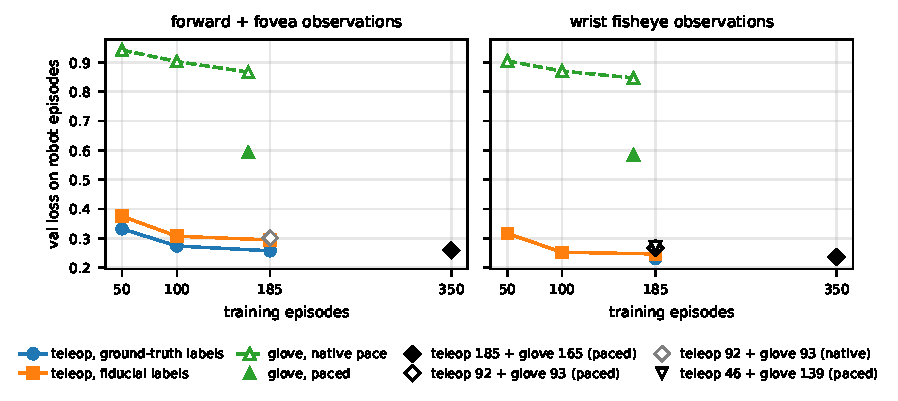
\includegraphics[width=0.62\linewidth]{fig/scaling.pdf}
  \caption{Validation loss on the robot's held-out episodes vs training-set size. Ground-truth and fiducial labels differ by a constant \SI{14}{\percent}; native-pace glove data stays a domain apart and pacing closes a third of the gap; the full co-trained corpora land at or below teleop-only, the equal-budget mixes above it.}
  \label{fig:scaling}
\end{figure}

\begin{figure}[t]
  \centering
  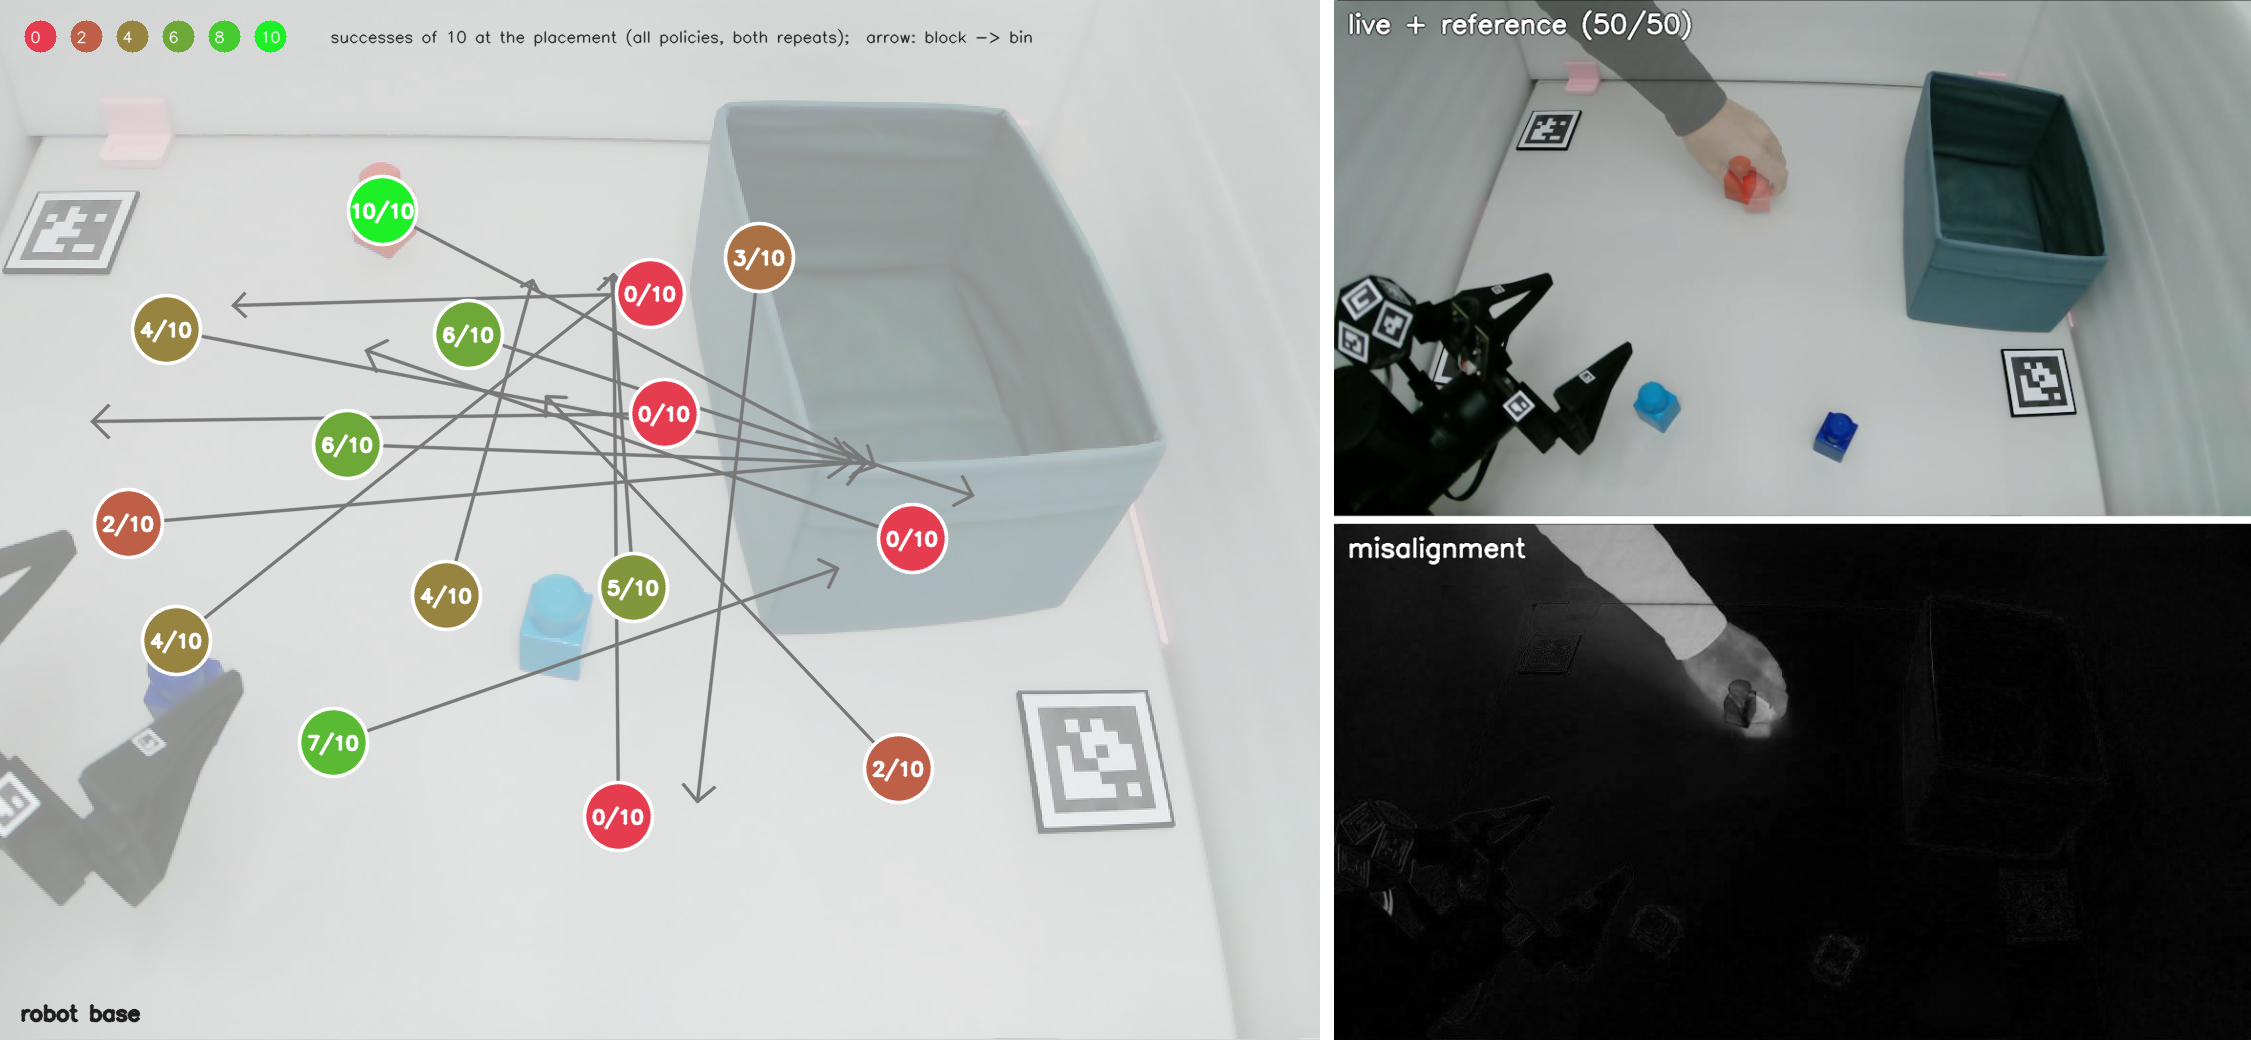
\includegraphics[width=0.66\linewidth]{fig/rollout_protocol.png}
  \caption{Rollout protocol. Left: the 15 placements (robot base bottom left); each disc is successes over all five policies and both repeats (of 10, red 0 to green 10); arrows point to each scene's bin. Right: before every trial the live view is blended with the scene's reference and shown as a misalignment image; the block is slid until the ghost disappears, so every policy and repeat meets the same scene to the pixel.}
  \label{fig:placements}
\end{figure}

\paragraph{Rollouts.}
Fifteen placements over the table, each run twice by every policy in shuffled order with the block re-placed to a saved reference (Fig.~\ref{fig:placements}), \SI{60}{s} budget, 30 trials per policy. The teleop-only wrist policy succeeds in 16/30 (Wilson 95\% CI 36--70\%); the co-trained policies in 14/30 (forward) and 12/30 (wrist), differences the paired exact McNemar test does not distinguish from zero ($p=0.77$, $0.29$). The two dilution policies succeed in 5/30 and 6/30, $-37$ and $-33$ points ($p=0.007$, $0.006$), losing in 7--8 of the 15 placements and winning one --- the opposite of what their validation losses, within \SI{10}{\percent} of the reference, suggest. The wrist arm's teleop-only curve is flat from 100 to 185 episodes (0.253 $\to$ 0.247, Fig.~\ref{fig:scaling}), so a loss near the reference is what 92 teleoperated episodes buy with or without glove data: loss on the robot's distribution does not predict rollouts once most of the corpus is glove data. The two repeats disagree in 7 of 75 policy--placement pairs, so outcomes are decided by the placement, and the effective sample is the 15 placements. Four placements at full reach were failed by every policy including the reference (success correlates with distance from the base, $\rho=-0.52$, not with carry length); the arms separate in the near two thirds, and not only by rate: three placements were solved by the co-trained policies and failed by the reference, one by the reference alone.

The failure modes split by camera. The forward-camera co-trained policy fails by never closing on the block (10 of 16 failures) and is otherwise the fastest (median \SI{20.7}{s} to success against \SI{28.2}{s}; joint speed \SI{21}{\percent} higher) although it trained on the same paced episodes as the wrist mix, whose speed equals the reference's: the speed comes from the view. The wrist policies close and then lose the block: counting a grasp as partial success (Table~\ref{tab:policies}, ``grasped'') the co-trained policy and the half-teleop mix are level with the reference, but they convert 43\% and 23\% of their grasps into the bin against 62\%. Glove data helps the reach and close; what it costs is the hold. The wrist videos say how: in every successful carry of the co-trained wrist policy the bin stays in the fisheye's view, and in every drop it is out of view, after which the policy hesitates and commands the release (7 of 16 drops, against 2 of 10 for the reference, whose drops are slips with the jaws commanded shut). The teleop-only policy carries blind for up to \SI{4}{s}; the co-trained one has lost that. Two hypotheses, not settled here: the teleop policy bridges the blind stretch from joint state, which maps onto the bin consistently in teleoperated data but not in glove episodes (joint actions from IK on a human hand path); or the paced corpus (one duplicated frame in four, human-speed motion blur) shifts the image distribution enough to cost it that habit. The forward camera was bumped by about \ang{3} during three placements and realigned; without those six trials the forward co-trained policy is 12/24.

%===============================================================================
\section{Limitations and what is next}
\label{sec:discussion}
Hardware \citep{yamumi2026} and software \citep{forwardcamumi2026} are open; a third party has built a unit and forked the design \citep{tinyumi2026}. The usable opening is \SI{75}{mm} of the \SI{86}{mm} mechanism, set by the span of thumb and fingers; the wrist cable can get in the way; a hard squeeze flexes the handle plate (the width label is measured, so unaffected); from one fixed viewpoint the hand hides the ball at grasp, hence the back markers (pose in 85\,\% of frames with them, 60\,\% without), and a head-worn second camera, once focused, solves it in \SI{99}{\percent} of frames. That points at what is next: we are testing whether the glove can lose its electronics altogether, with one head-worn camera as the only collection device --- no cables, nothing to synchronise --- labelling the glove from a moving viewpoint and doubling as the policy's input; the label stack already runs on head-camera footage \citep{forwardcamumi2026}.

%===============================================================================
\bibliography{refs}

\end{document}
